\chapter{Quantum machine learning}

\section{Data encoding}

\section{Quantum neural networks}

\subsection{QNNs vs NNs}\label{sec:qnn-vs-nn}
Fisher's iris dataset is perhaps the most used dataset for classification in statistics, containing samples of three different species of iris flowers. For each species, there are 50 samples, each with four features: sepal length, sepal width, petal length, and petal width. Like in \cite{abbas2021}, only the two first species are considered, which happen to be linearly separable in the feature space.

To compare the performance of the QNN and the NN, architectures suited for binary classification parametrised by exactly 8 parameters are used. The QNN structure is shown in \cref{fig:qnn_vs_nn_models}. The four dimensional input data $\bm{x}$ is mapped to some quantum state $\ket{\psi{\bm{x}}}$ using the ZZFeatureMap with two repetitions, which is a second-order Pauli-Z evolution circuit. This feature map is essentially a mix of rotation around the Z axis parametrised by the input features or functions thereof and CNOT and Hadamard gates. The quantum state is then evolved by the RealAmplitudes ansatz. All four qubits a rotated in the Y direction by some parameter before CNOT-gates are applied pairwise, for a final parametrised rotation in the Y direction, for a total of 8 parameters. For details on the components, see Qiskit's documentation \cite{qiskit} or the original paper \cite{abbas2021}. The parity of the output 4-bit string is interpreted as the prediction, and with 100 shots used, the model gave a probability for each of the two iris classes. Both exact simulations and noisy simulations were performed, with the latter using noise modelled after the 27-qubit IBM Montreal architecture, the actual hardware used in the original paper.

\begin{figure}
    \centering
    \begin{quantikz}
        \lstick[wires=4]{$\ket{0}^{\otimes 4}$} & \gate[wires=4]{\text{ZZFeatureMap}(\bm{x})} & \gate[wires=4]{\text{RealAmplitudes}(\bm{\theta})} & \meter{} \\
        & & & \meter{} \\
        & & & \meter{} \\
        & & & \meter{} \\
    \end{quantikz}
    \caption{Structure of the QNN used for classification of the iris dataset. The first block maps the input data $\bm{x}$ to the quantum state $\ket{\psi(\bm{x})}$. The second block is the variational circuit, parametrised by $\bm{\theta}$, a vector with eight components. Finally, all qubits are measured, where the parity is interpreted as the prediction.}
    \label{fig:qnn_vs_nn_models}
\end{figure}

The classical neural network was a standard feed-forward model, with a 4-1-1-1-2 layered structure without biases, giving a total of 8 parameters. The activation functions were leaky ReLUs,
\begin{equation}
    \text{LeakyReLU}(x) = \begin{cases}
        x     & x \geq 0 \\
        0.01x & x < 0
    \end{cases},
\end{equation}
and the output layer used a softmax activation function.

Both models were implemented using PyTorch, with the QNN being implemented using Qiskit's PyTorch interface. Consequently, the models could be trained in the exact same manner, using the Adam optimiser with a learning rate of 0,1. The models were trained for 100 epochs, with the loss function being cross-entropy.

For validation, 10-fold cross-validation was used. That is, the dataset was split into 10 equal parts or \textit{folds}. Each fold us used as the validation set once, their accuracies being recorded during the training with the other nine folds. The mean accuracy over the 10 folds was used for the final performance metric, shown in \cref{fig:iris_training}.

As in the original paper, the QNN converges much quicker and more consistently, with an out-of-fold accuracy of 100\% for all ten folds. The NN, on the other hand, requires more iterations to converge and does not always do so. In some cases, the model diverges and only predicts one class, which is why the out-of-fold accuracy is not 100\% for all folds.


\begin{figure}
    \centering
    \begin{tikzpicture}
        \begin{axis}[
                width=0.8\textwidth,
                xlabel={Iteration},
                ylabel={Out of fold accuracy},
                grid = major,
                legend pos=south east,
                legend cell align={left},
                % add 1 to x axis
            ]
            \addplot[mark=none, color=blue] table[x expr=\coordindex+1, y index=3, col sep=comma] {../code/iris/results/mean.csv};
            \addplot[mark=none, color=red] table[x expr=\coordindex+1, y index=2, col sep=comma] {../code/iris/results/mean.csv};
            \addplot[mark=none, color=green] table[x expr=\coordindex+1, y index=1, col sep=comma] {../code/iris/results/mean.csv};
            \legend{
                Noisy QNN,
                Exact QNN,
                Classical NN
            }
        \end{axis}
    \end{tikzpicture}
    \caption{Mean accuracy during training for the iris dataset using 10-fold cross validation. All models have 8 parameters and are trained using the Adam optimiser with a learning rate of 0.1, using cross-entropy as the loss function. Due to the computational cost, the noisy (simulated IBM Montreal backend) QNN was only trained for 10 epochs.}
    \label{fig:iris_training}
\end{figure}

\subsection{Quantum convolutional neural networks}
Quantum convolutional neural networks work similarly to classical convolutional networks. Through iterated convolution and pooling layers where only 'near' features affect each other, the total amount of parameters is reduced relative to fully connected networks, and the CNN tends to learn more local features. This makes them well suited for image classification, where the significant features are often spatially correlated. The reduced amount of parameters also makes them suitable for quantum hardware, and they have shown desireable properties with regard to avoiding barren plateaus \cite{pesah2021}.

To implement a quantum CNN, Qiskit's online tutorials was closely followed \cite{qiskit_qcnn}. Being limited to few qubits, images with resolution $2\times4$ were generated, containing either vertical or horizontal with some Gaussian noise. \Cref{fig:qcnn_data} shows examples thereof. The task of the QCNN was to classify the images as either vertical or horizontal lines.

\begin{figure}
    \centering
    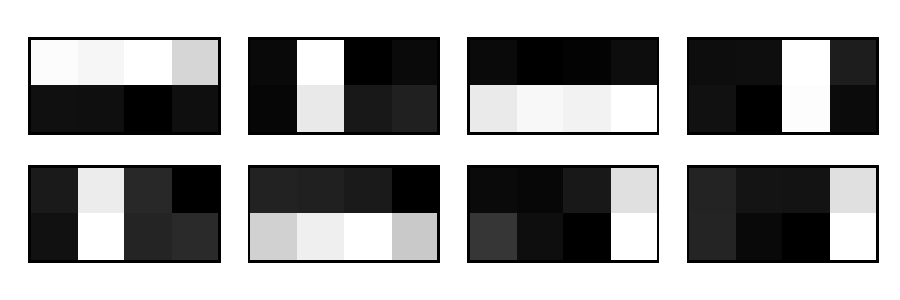
\includegraphics[width=\textwidth]{../code/qcnn/data.pdf}
    \caption{Data for the QCNN. With a total of 64 training images and 16 for testing, they form balanced dataset of $2\times4$ pixels, with either a vertical or horizontal line encoded as $1$ and $-1$. The images are generated with some Gaussian noise.}
    \label{fig:qcnn_data}
\end{figure}


First, data is encoded using Qiskit's ZFeatureMap; each of the nine pixels of the image is mapped to a qubit through two repetitions of the Hadamard gate and Z-rotations parametrised by the pixel value being applied, in circuit notation:

\begin{center}
    \begin{quantikz}
        \lstick{$\ket{0}$} & \gate{H} & \gate{R_Z(x_1)} & \gate{H} & \gate{R_Z(x_1)}  \\
        \lstick{$\ket{0}$} & \gate{H} & \gate{R_Z(x_2)} & \gate{H} & \gate{R_Z(x_2)}  \\
        \lstick{\vdots} \\
        \lstick{$\ket{0}$} & \gate{H} & \gate{R_Z(x_n)} & \gate{H} & \gate{R_Z(x_n)}  \\
    \end{quantikz}
\end{center}



The convolution layers act with pairwise parametrised rotations of neighbouring qubits, also wrapping around, entangling the first and last qubits through various CNOT gates and both parametrised and fixed Z and Y rotations. Thereafter, pooling layers halve the active qubit counts by parametrised rotations and CNOT gates. For the final layer, the sole remaining qubit is measured, and the result is interpreted as the prediction. In total, the circuit appears as

\begin{center}
    \begin{quantikz}
        \lstick[wires=8]{$\ket{0}^{\otimes 8}$} &
        \gate[wires=8, disable auto height]{{\rotatebox{90}{\text{ZFeatureMap}}}} &
        \gate[wires=8, disable auto height]{{\rotatebox{90}{\text{Convolution}}}} &
        \gate[wires=8, disable auto height]{{\rotatebox{90}{\text{Pooling}}}} & \qw{}& \qw{}& \qw{}& \qw{} & \qw{}
        \\
        & \qw{}& \qw{}& \qw{}& \qw{}& \qw{}& \qw{}& \qw{}& \qw{}\\
        & \qw{}& \qw{}& \qw{}& \qw{}& \qw{}& \qw{}& \qw{}& \qw{}\\
        & \qw{}& \qw{}& \qw{}& \qw{}& \qw{}& \qw{}& \qw{}& \qw{}\\
        & & & &
        \gate[wires=4, disable auto height]{{\rotatebox{90}{\text{Convolution}}}} &
        \gate[wires=4, disable auto height]{{\rotatebox{90}{\text{Pooling}}}} & \qw{} & \qw{} & \qw{}
        \\
        & \qw{}& \qw{}& \qw{}& \qw{}& \qw{}& \qw{}& \qw{}& \qw{}\\
        & & & & & &
        \gate[wires=2, disable auto height]{{\rotatebox{90}{\text{Conv}}}} &
        \gate[wires=2, disable auto height]{{\rotatebox{90}{\text{Pooling}}}} & \qw{}

        \\
        & & & & & & & & \meter{} \\
    \end{quantikz}
\end{center}


As in Qiskit's guide, training was done using thee COBYLA optimiser\footnote{Constrained Optimisation BY Linear Approximation.} which does not use gradients. The accuracies and loss (mean square error) during training is shown in \cref{fig:qcnn_loss}. Like in \cref{sec:qnn-vs-nn}, noise is modelled after the IBM Montreal hardware. The networks were trained for 1000 epochs, and while neither reached full accuracy, the losses shrunk, indicating at least increased certainty in the predictions. Interestingly, the noisy simulation appears to yield better predictions, despite suffering from higher losses during training.


\begin{figure}
    \centering
    \begin{subfigure}{\textwidth}
        \centering
        \begin{tikzpicture}
            \begin{axis}[
                    width=0.8\textwidth,
                    xlabel={Iteration},
                    ylabel={Loss (MSE)},
                    % legend pos=north west,
                    % legend style={at={(0.5,1.03)},anchor=north},
                    grid=major,
                ]
                \addplot[mark=none, color=red] table[x=iteration, y=loss, col sep=comma] {../code/qcnn/noisy.csv};
                \addplot[mark=none, color=blue] table[x=iteration, y=loss, col sep=comma] {../code/qcnn/exact.csv};
                \legend{
                    Noisy QCNN,
                    Exact QCNN,
                }
            \end{axis}
        \end{tikzpicture}
    \end{subfigure}
    \begin{subfigure}{\textwidth}
        \centering
        \begin{tikzpicture}
            \begin{axis}[
                    width=0.8\textwidth,
                    xlabel={Iteration},
                    ylabel={Accuracy},
                    % legend pos=north west,
                    % legend style={at={(0.5,1.03)},anchor=north},
                    grid=major,
                    legend pos=south east,
                ]
                \addplot[mark=none, color=red] table[x=iteration, y=training_acc, col sep=comma] {../code/qcnn/noisy.csv};
                \addplot[mark=none, color=red, dashed] table[x=iteration, y=test_acc, col sep=comma] {../code/qcnn/noisy.csv};
                \addplot[mark=none, color=blue] table[x=iteration, y=training_acc, col sep=comma] {../code/qcnn/exact.csv};
                \addplot[mark=none, color=blue, dashed] table[x=iteration, y=test_acc, col sep=comma] {../code/qcnn/exact.csv};
                \legend{
                    Noisy training,
                    Noisy test,
                    Exact trainin,
                    Exact test,
                }
            \end{axis}
        \end{tikzpicture}
    \end{subfigure}
    \caption{Training of the QCNN. The first plot shows the loss (mean square error) during training, while the second plot shows the accuracy on the training and test sets. The red curves are for the noisy model, while the blue curves are for the exact model. The dashed curves are for the test set.}
    \label{fig:qcnn_loss}
\end{figure}


